\documentclass[../../lectures.tex]{subfiles}

\begin{document}

\chapter{Файловые системы}

\section{Носители}
\subsection{HDD}
\centerimage{hard-disk.jpg}{Жесткий диск}{1}
\begin{itemize}
    \item Обороты в минуту($O$) --- 5400, 7200, 10000, ...
    \item $\frac{1}{2 * O}$ --- минимальное время доступа (случайное чтение)
    \item В мире Unix не существует дефрагментации (ОС должна сама заботиться)
    \item Время отказа (\textbf{MTBF} --- min time before failure) --- условное 
          количество циклов наработки до отказа
    \item На \textbf{server} --- сутки, \textbf{desktop} --- часы (разница примерно в 3 раза, 
          если одно и то же число циклов)
    \item Плюсы: стоимость, объем
    \item Минусы: время доступа, надежность
\end{itemize}

\subsection{SSD}
\begin{itemize}
    \item \textbf{SATA} и \textbf{NVME} --- протоколы для дисков
    \item \textbf{NVME} --- новомодная штука для \textbf{SSD}
    \item Плюсы: время доступа
    \item Минусы: надежность, стоимость, объем
\end{itemize}

\subsection{Общее}
\begin{itemize}
    \item \textbf{IOPS} --- input/output operations per second
        
          Показатель применяется для сравнения, например, какого-нибудь \textbf{HDD} с \textbf{SSD}
    \item \textbf{seek} --- рандомное чтение (512 байт)
    \item Минимум информации: сектор --- 512 байт -> 4096 байт
    \item Чтение одного байта равносильно чтению всего сектора с этим байтом
    \item Запись одного байта --- считать один сектор, заменить байт и записать один сектор
    \item Аналогия --- процессор-память --- \textbf{cacheline} 
        
         (кэшируется линиями, а на диск записывается и считывается секторами)
\end{itemize}

\section{Быстродействие}
\subsection{Интересные числа}
\begin{center}
Числа, которые должен знать каждый программист
\\~\\
\begin{tabular}{| l | l |}
    \hline
    Cycle                            & 1   ns \\ \hline
    Main memory reference            & 100 ns \\ \hline
    Read 4K randomly from SSD        & 150 us \\ \hline
    Read 1 MB sequentially from SSD  & 1   ms \\ \hline
    Disk seek                        & 10  ms \\ \hline
    Read 1 MB sequentially from disk & 20  ms \\ \hline
\end{tabular}
\end{center}
\subsection{Выводы для HDD}
\begin{itemize}
    \item Читать нужно последовательно
    \item Обращения к диску следует минимизировать
    \item Стоимость доступа сильно дороже передачи данных
\end{itemize}

\section{Structure packaging}
Сколько будет занимать памяти следующая структура?

\code{hole1.c}{C}

Ответ: 32 байта, так как $b$ и $d$ будут выравнены по MAX\_ALLIGNMENT

Очевидное решение проблемы:

\code{hole2.c}{C}

Данная структура будет занимать 24 байта на x86\_64.

\section{Алгоритмы элеватора}
\textcolor{blue}{\href{https://slideplayer.com/slide/5209336}{Ссылка на презентацию}}
\begin{enumerate}
    \item SLIDE 6

          Алгоритмы элеватора обрабатывают последовательности запросов к диску (переупорядочивают их)
    \item SLIDE 7

          \textbf{FCFS} (FIFO)

          Самый простой и медленный
    \item SLIDE 8-9

          \textbf{SSTF} (Shortest Seek Time First)

          Сортировка (очередной запрос определяется наименьшим временем seek)
    \item SLIDE 10 - \dots

          Различные способы упорядочивания (\textbf{SCAN})
\end{enumerate}

\section{Файл}
\begin{itemize}
    \item Абстракция для данных (для Kernelspace)
    \item Последовательность байтов (для Userspace)
    \item Формат не определен
    \item \textbf{Unix} --- все есть файл (абстракция-интерфейс внутри ядра)
    \item Типы файлов 
          \begin{itemize}
            \item regular
            \item directory
            \item symlink
            \item socket, fifo
            \item character device, block device
          \end{itemize}
\end{itemize}

\section{Директория}
\begin{itemize}
    \item Содержит имена находящихся в ней файлов
    \item $.$ --- ссылка на текущую
    \item $..$ --- ссылка на родителя
    \item \shell{cd} --- сменить директорию
    \item \shell{pwd} --- текущая директория
    \item \shell{ls} --- формирование дерева
    \item \shell{find} --- поиск
    \item \emph{filename vs pathname}: \shell{realpath}
\end{itemize}
\subsection{Права --- просто числа}
\begin{itemize}
    \item \shell{view /etc/passwd}
    \item \shell{view /etc/group}
    \item \shell{id} - показывает идентификаторы того, кто ее вызывал
    \item \shell{execute} --- search
    \item \shell{read} --- directory listing
    \item \shell{write} --- changing directory
    \item Темные директории (переход в директорию внутри директории, для который ты не можешь посмотреть все файлы)
    \item Права rwx (read, write, execute)
    \item \shell{chmod} --- меняет права доступа
          
          \shell{chmod 123} --- 1 - user, 2 - group, 3 - other
    \item У процесса есть информация о том, кто его запустил
    \item \textbf{SGID} (\textbf{S}et \textbf{G}roup \textbf{ID} up on execution)

          Специальный тип прав, который временно выдается запускающему (у него теперь права группы на файл/директорию)
\end{itemize}
\subsection{sticky bit}
\begin{itemize}
    \item Изменение поведения при создании нового файла
    \item /tmp
    \item Создаешь директорию со \emph{sticky bit} и все, кто создают файлы в этой директории имеют на них права
\end{itemize}

\section{Иерархия}
\begin{figure}[H]
\begin{minipage}[c]{0.5\linewidth}
\centering
\begin{itemize}
    \item $/$
        \begin{itemize}
            \item bin/
            \item dev/
            \item etc/
            \item sbin/
            \item home/
            \item var/
            \item usr/
                \begin{itemize}
                    \item bin/
                    \item sbin/
                \end{itemize}
            \item tmp
        \end{itemize}
\end{itemize}
\end{minipage}
\hspace{0.5cm}
\begin{minipage}[c]{0.37\linewidth}
\centering
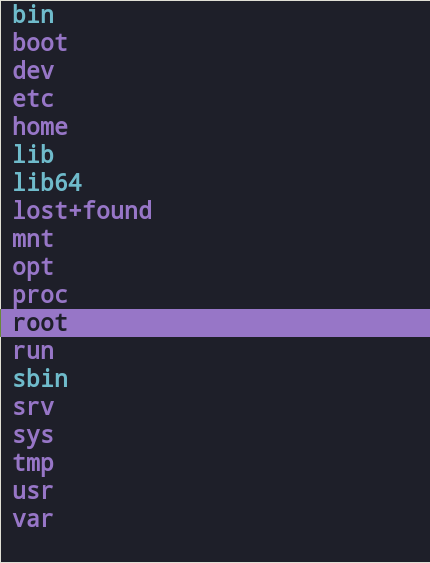
\includegraphics[width=\textwidth]{images/root.png}
\caption{Типичный вид корня в Linux}
\end{minipage}
\end{figure}

\section{Монтирование}
\begin{itemize}
    \item Есть корень и есть узлы, в которые можно монтировать другие файловые системы (часть из них виртуальная)
    \item \shell{mount}
    \item Для $/$ обычно используется \textbf{ext4} (использует журналирование)
    \item Для /boot может использоваться \textbf{ext2} --- так как это более проверено временем (на Ubuntu)
    \item Файловая система для узла --- это не константа, ее можно менять
    \item \shell{df - h}, \shell{du -hs}
\end{itemize}

\section{Inode}
\begin{itemize}
    \item Директория задает mapping имени файла в его inode
    \item \shell{ln}
    \item Hardlink --- существует в рамках одной файловой системы
    \item Softlink(symlink) --- text string
    \item \shell{stat} --- информация о файле
    \item \emph{atime} --- время последнего доступа
    \item \emph{ctime} --- изменение мета-информации
    \item \emph{mtime}--- изменение содержимого файла
    \item inode корневой файловой системы фиксирован --- 2
\end{itemize}

\section{Проход по пути}
\begin{itemize}
    \item Рекурсивный процесс (увеличиваем индекс при проходе в глубину)
    \item Количество seek по диску зависит от длины пути
    \item namei (name-innode) --- lru-cache (файл <--> номер inode)
\end{itemize}

\section{Атрибуты процесса}
\begin{figure}[H]
\begin{minipage}[c]{0.5\linewidth}
\centering
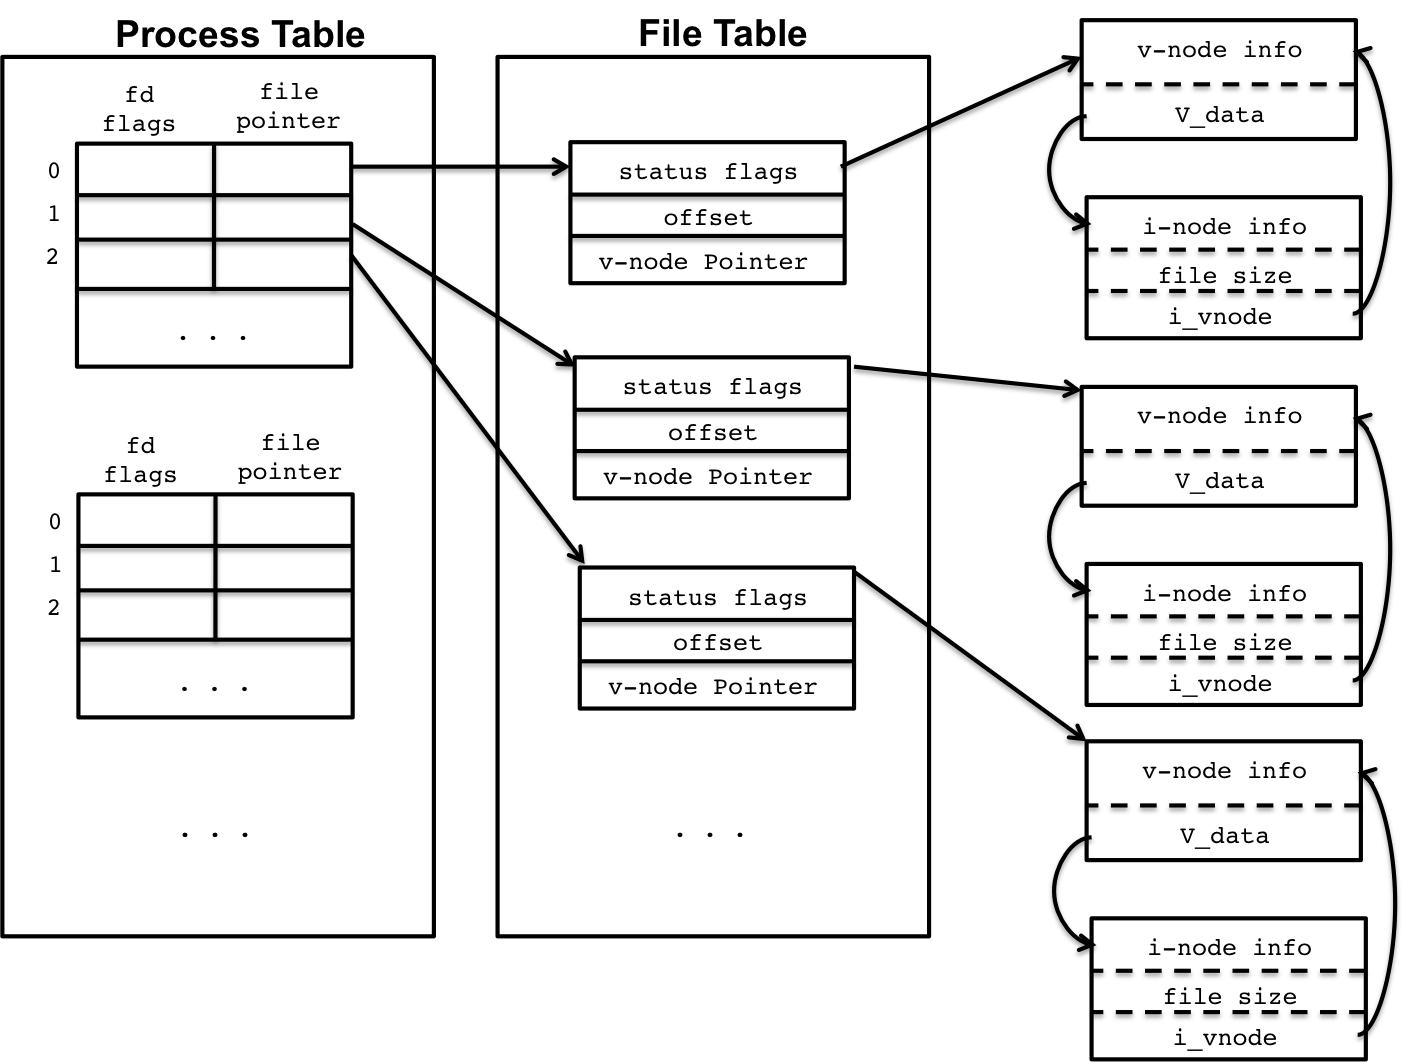
\includegraphics[width=\textwidth]{images/kernel-datastructures.png}
\caption{Structures of Kernel}
\end{minipage}
\hspace{0.5cm}
\begin{minipage}[c]{0.5\linewidth}
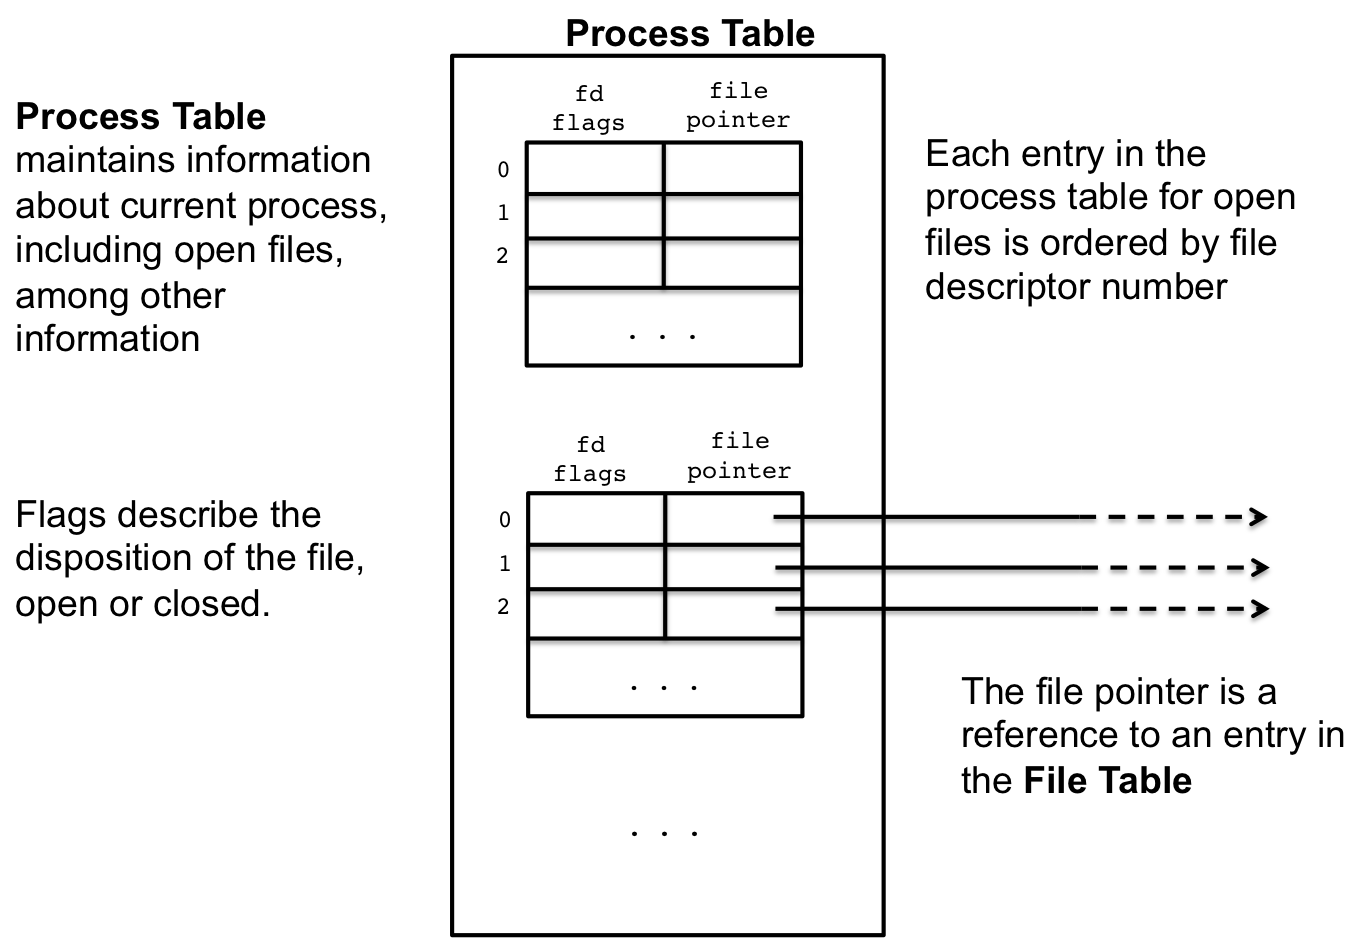
\includegraphics[width=\textwidth]{images/process-table.png}
\caption{Processes}
\end{minipage}
\end{figure}
\begin{figure}[H]
\begin{minipage}[c]{0.5\linewidth}
\centering
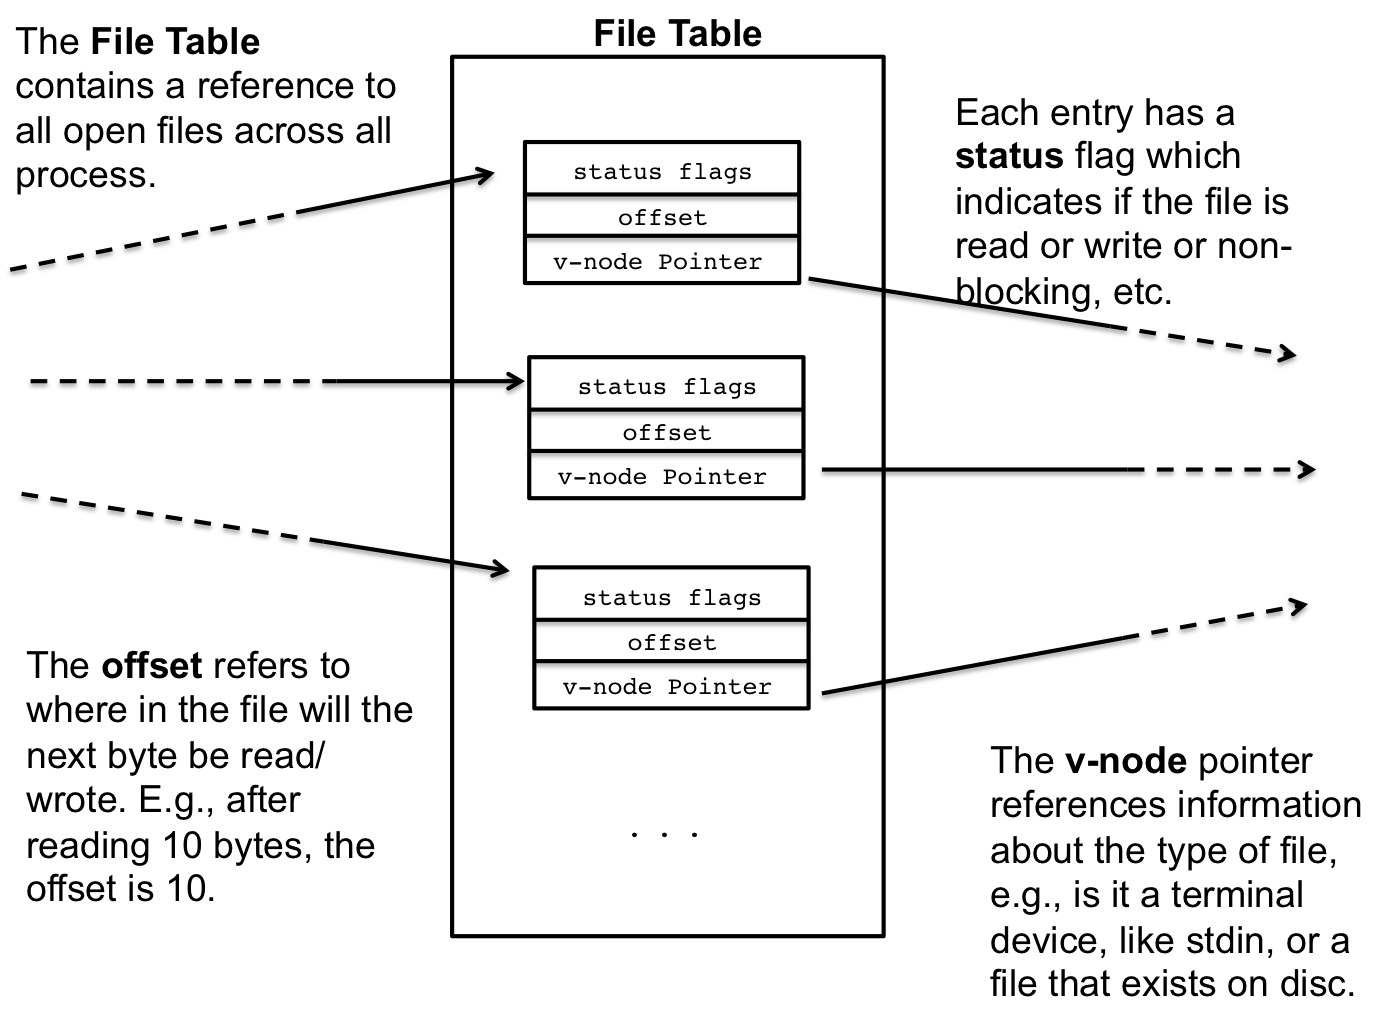
\includegraphics[width=\textwidth]{images/file-table.png}
\caption{Files}
\end{minipage}
\hspace{0.5cm}
\begin{minipage}[c]{0.5\linewidth}
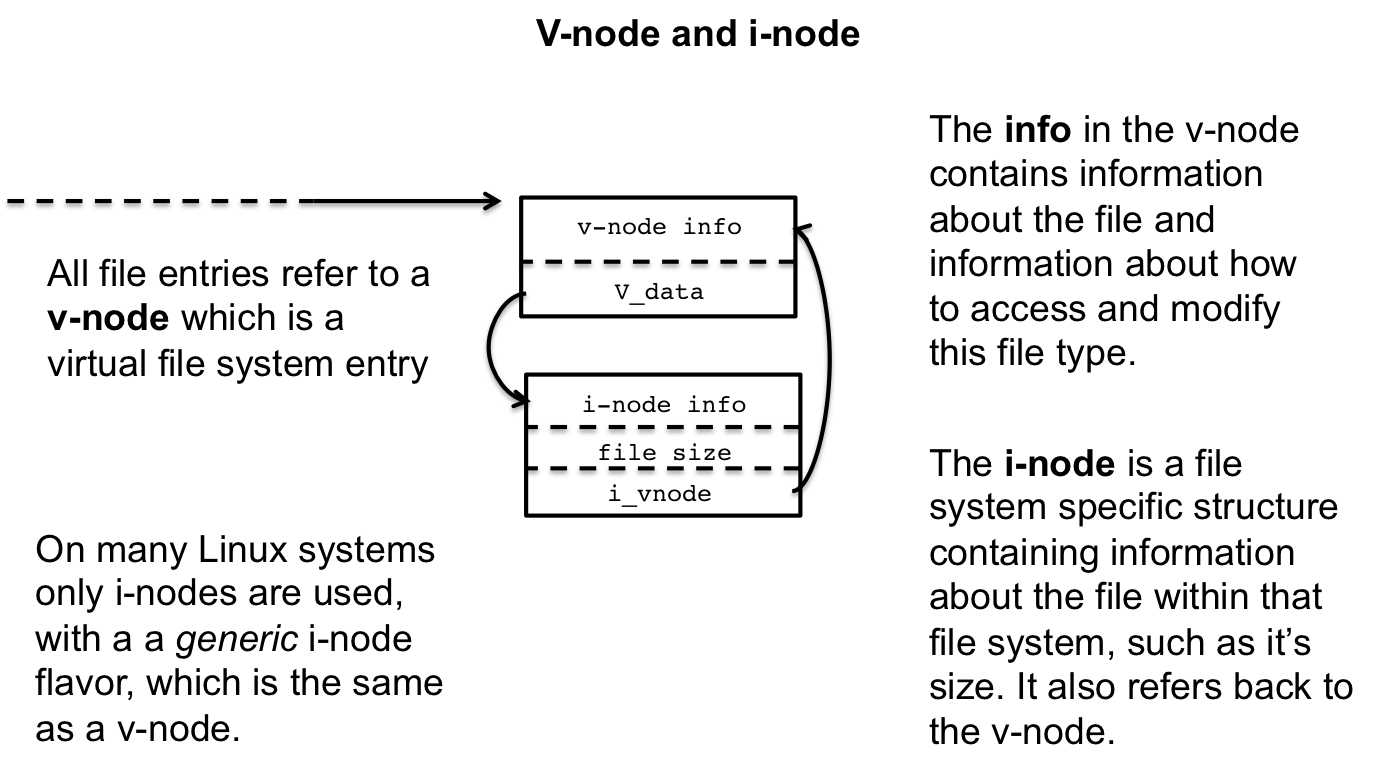
\includegraphics[width=\textwidth]{images/vnode-table.png}
\caption{Vnode and Inode}
\end{minipage}
\end{figure}
\todo{???}

\section{Диски}
\begin{figure}[H]
\begin{minipage}[c]{0.6\linewidth}
\centering
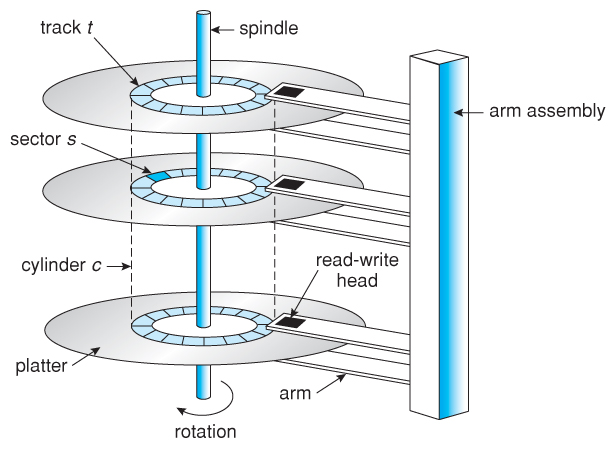
\includegraphics[width=\textwidth]{images/disk-mechanism.jpg}
\caption{Устройство диска}
\end{minipage}
\begin{minipage}[c]{0.4\linewidth}
\centering
Устройство диска
\begin{itemize}
  \item сектор
        \begin{itemize}
            \item header: метаданные для контроллера диска
            \item данные
            \item trailer: ECC
        \end{itemize}
  \item цилиндр
  \item пластина
  \item трэк
  \item шпиндель
\end{itemize}
\end{minipage}
\end{figure}
\begin{itemize}
    \item При записи данных на диск в сектора считаем и записываем \textbf{ECC},
          при чтении считаем и затем сверяем (пытаемся исправить, если не сошлось)

    \item \textbf{CLV} --- Constant Linear Velocity(\textbf{CDROM})
    \item \textbf{CAV} --- Constant Angular Velocity(\textbf{HDD})
    \item На внешних цилиндрах больше секторов, чем на внутренних 
          => чем ближе к центру тем меньше скорость нужна (CD)
    \item На жестких дисках --- постоянная угловая скорость 
          (в центре больше плотность)
    \item \emph{Partitioning} --- разделение диска на несколько 
          логических частей (партиции, на каждой своя файловая система),
          они трактуются как "отдельные" диски
    \item Существует другой подход - "собственная" файловая система 
          на "сыром" диске (MySQL)
    \item Современный контроллер жесткого диска может находить механически поврежденные блоки (bad blocks) и делать remap их на некоторые запасные (sector sparing: replace bad sectors with spare)
    \item \shell{man 1 badblocks}
    \item Bootblock --- bootstrap program at fixed location
    \item \textbf{MBR} --- master boot record --- boot code + partition table
\end{itemize}

\section{RAID}
Redundant Arrays of Independent Disks (Избыточный массив независимых дисков)

\begin{figure}[H]
\begin{minipage}[c]{0.5\linewidth}
\centering
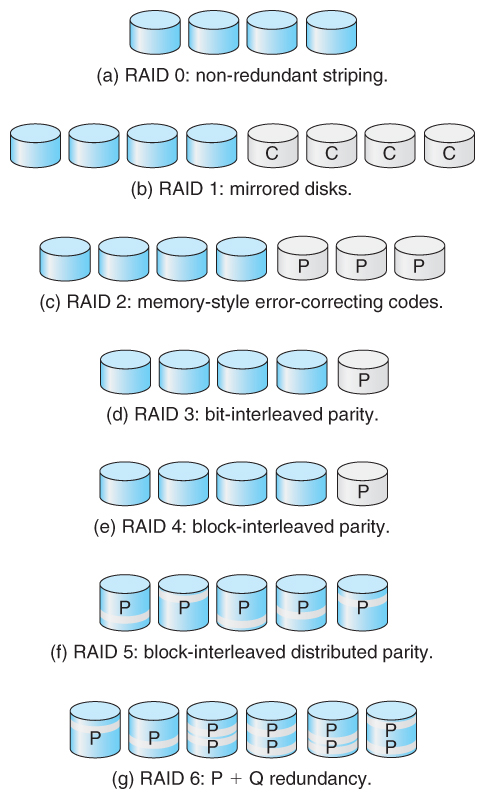
\includegraphics[width=\textwidth]{images/raid-levels.jpg}
\caption{RAID levels}
\end{minipage}
\begin{minipage}[c]{0.5\linewidth}
\centering
\begin{itemize}
    \item Reilability (надежность, hacks for more long time of complex usage)
    \item Perfomance (striping, суммирование \textbf{IOPS})
    \item Levels:
        \begin{itemize}
            \item \textbf{0} --- pure striping (1 блок на 1 диске, 2 блок на 2 диске и т.д. --- один диск вышел из строя --- fail)
            \item \textbf{1} --- pure mirroring (пара дисков, данные продублированы)
            \item \textbf{0 + 1, 1 + 0}
            \item \textbf{2, 3, 4, 5} --- используются не так часто (хранение доп. данных)
        \end{itemize}
    \item Rebuild --- падает производительность
    \item Hardware RAID --- проблемы: "залоченность" на производителе (vendor lock in), драйвера, как правило, не очень
    \item Software RAID --- гипотетически медленно, но на практике нужная производительность достигается
    \item У аппаратных RAID --- есть батарейка, которая "улучшает" производительность 
          (сначала на батарейку, потом на диск, когда будет удобно)
    \item \todo{Байка про SpaceWeb}
\end{itemize}
\end{minipage}
\end{figure}

\newpage
\section{Организация файловых систем}
Структура директорий: связный список или хэш-таблица

smart (\shell{smartctl}) --- оценка диска на практике

Свободные сектора
\begin{enumerate}
    \item Bit Vector --- fast, space usage
    \item Список
\end{enumerate}

\begin{center}\textbf{Выделение памяти (allocation)}\end{center}

\begin{figure}[H]
\begin{minipage}[c]{0.47\linewidth}
\centering
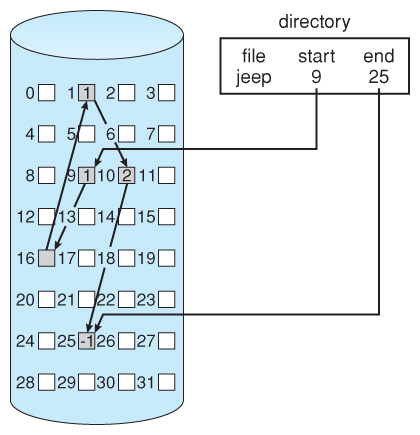
\includegraphics[width=\textwidth]{images/linked-allocation.jpg}
\caption{Linked allocation}
\end{minipage}
\hspace{0.5cm}
\begin{minipage}[c]{0.5\linewidth}
\centering
\textbf{Линейное}
\begin{itemize}
    \item Объект задается началом и концом (здесь возникают проблемы внешней и внутренней фрагментации)
    \item Линейное чтение, меньше обращений
    \item Perfomance: sequential, random
\end{itemize}
\end{minipage}
\end{figure}

\begin{figure}[H]
\begin{minipage}[c]{0.47\linewidth}
\centering
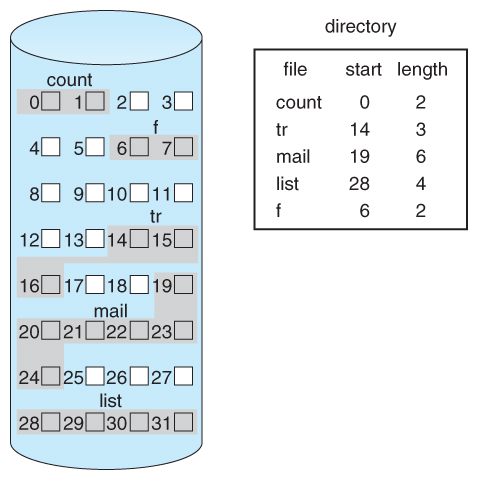
\includegraphics[width=\textwidth]{images/contiguous-allocation.jpg}
\caption{Contiguous allocation}
\end{minipage}
\hspace{0.5cm}
\begin{minipage}[c]{0.5\linewidth}
\centering
\textbf{Список}
\begin{itemize}
    \item В каждом "блоке" указатель на следующий
    \item Плюсы: решает проблему внешней фрагментации
    \item Минусы: надежность, прыгаем по памяти
    \item Perfomance: sequential, awful random
\end{itemize}
\end{minipage}
\end{figure}

\begin{figure}[H]
\begin{minipage}[c]{0.47\linewidth}
\centering
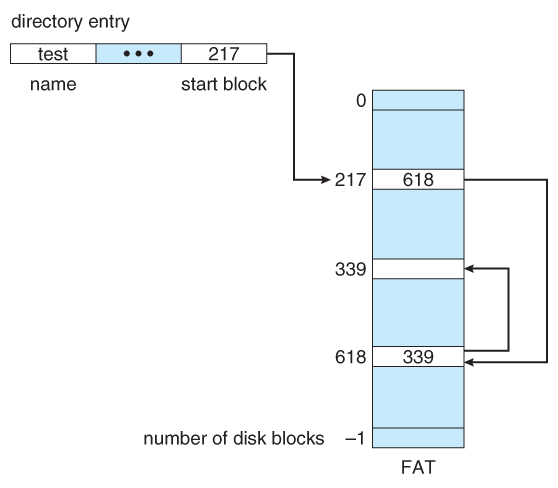
\includegraphics[width=\textwidth]{images/fat-table.jpg}
\caption{FAT allocation}
\end{minipage}
\hspace{0.5cm}
\begin{minipage}[c]{0.5\linewidth}
\centering
\textbf{FAT}
\begin{itemize}
    \item Все ссылки хранятся в начале диска --- их можно эффективно кэшировать
    \item Улучшенный поиск
\end{itemize}
\end{minipage}
\end{figure}

\begin{figure}[H]
\begin{minipage}[c]{0.47\linewidth}
\centering
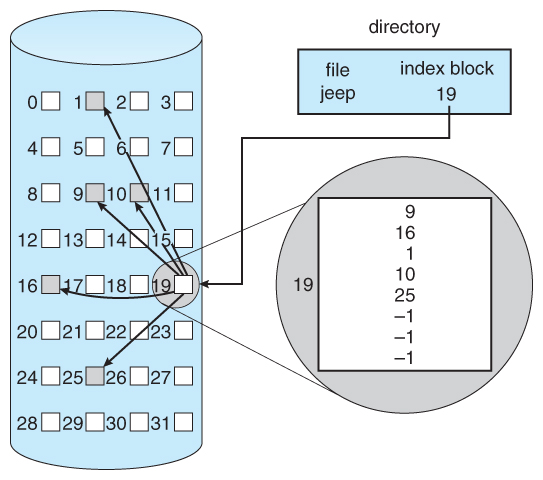
\includegraphics[width=\textwidth]{images/indexed-allocation.jpg}
\caption{Indexed allocation}
\end{minipage}
\hspace{0.5cm}
\begin{minipage}[c]{0.5\linewidth}
\centering
\textbf{Индексированное}
\begin{itemize}
    \item Отдельный блок для ссылок на данные
    \item Внутренняя фрагментация
\end{itemize}
\end{minipage}
\end{figure}

\begin{figure}[H]
\begin{minipage}[c]{0.47\linewidth}
\centering
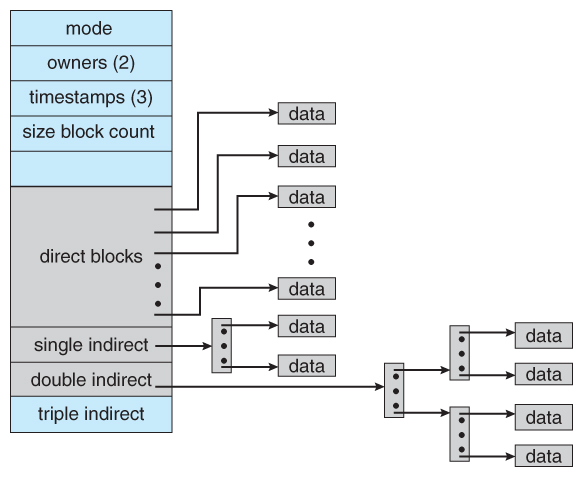
\includegraphics[width=\textwidth]{images/unix-inode.jpg}
\caption{UNIX allocation}
\end{minipage}
\hspace{0.5cm}
\begin{minipage}[c]{0.5\linewidth}
\centering
\textbf{UNIX}
\begin{itemize}
    \item Комбинированная
    \item Косвенная многоуровневая адресация
\end{itemize}
\end{minipage}
\end{figure}

\section{Файловые системы}
\begin{figure}[H]
\begin{minipage}[c]{0.6\linewidth}
\centering
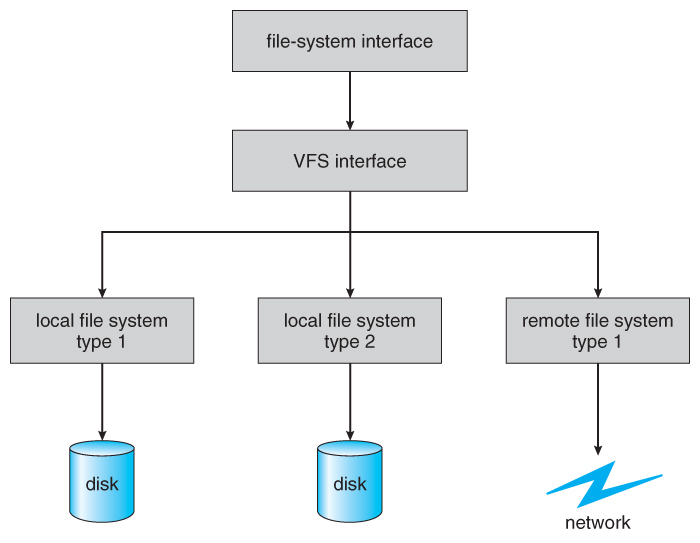
\includegraphics[width=\textwidth]{images/virtual-fs.jpg}
\caption{VFS}
\end{minipage}
\begin{minipage}[c]{0.4\linewidth}
\begin{itemize}
    \item \textbf{VFS}
    \item Сетевые
    \item Виртуальные
    \item На диске
    \item В памяти
\end{itemize}
\end{minipage}
\end{figure}

\section{Операции с файлами}
\begin{figure}[H]
\begin{minipage}[c]{0.25\linewidth}
\centering
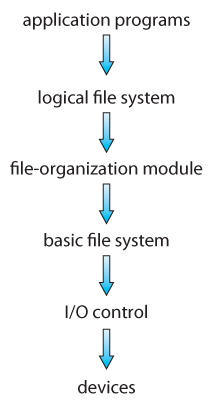
\includegraphics[width=\textwidth]{images/layered.jpg}
\caption{Layered}
\end{minipage}
\hspace{0.5cm}
\begin{minipage}[c]{0.75\linewidth}
\centering
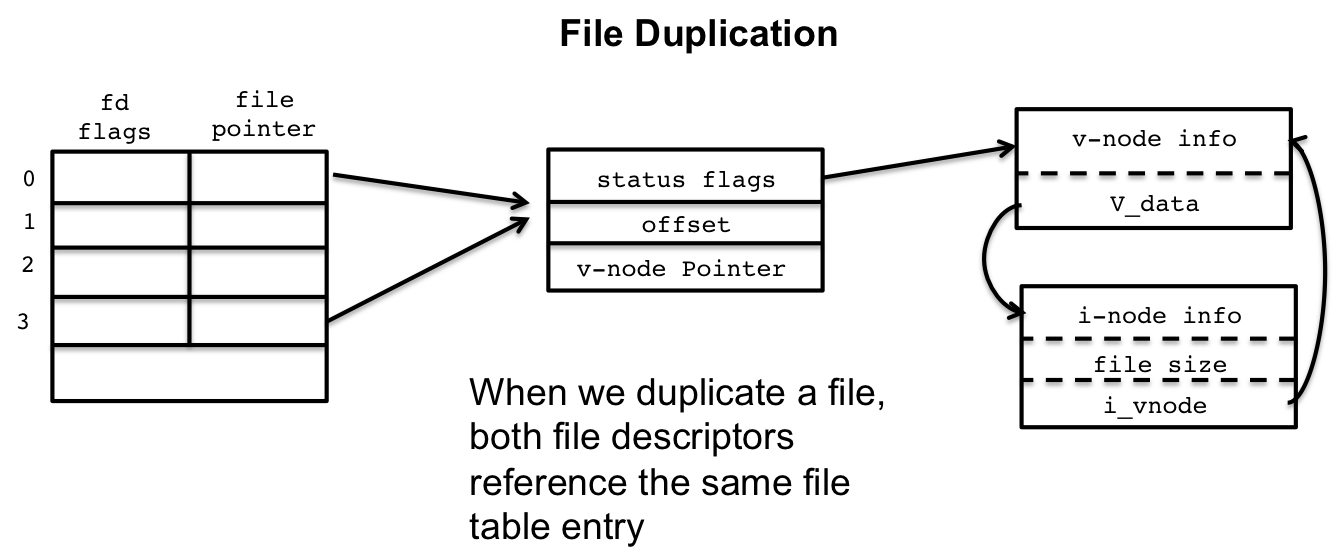
\includegraphics[scale=0.38]{images/dup.png}
\caption{Duplication}
~

~
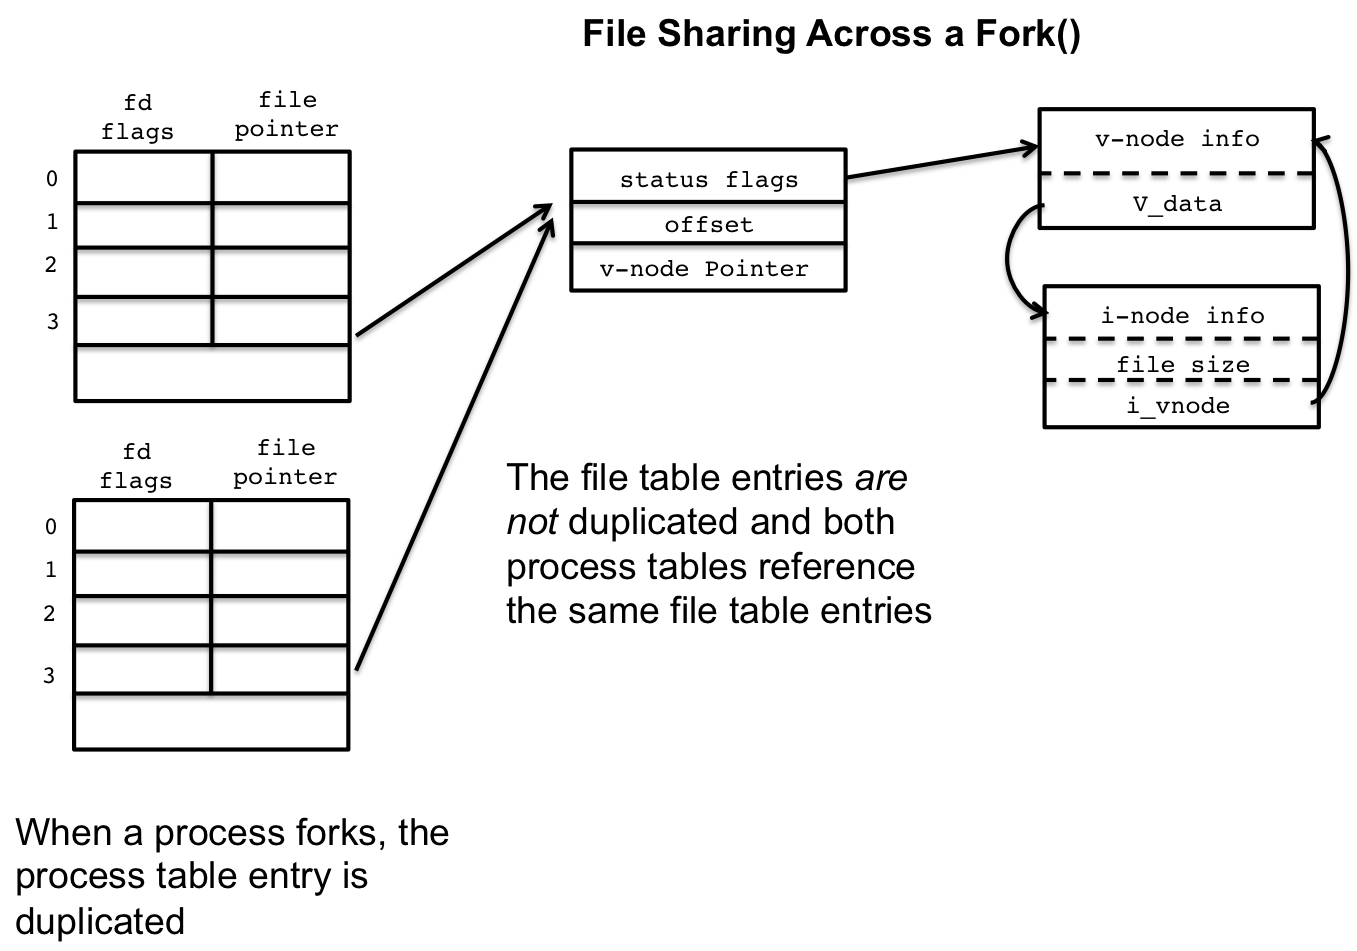
\includegraphics[scale=0.37]{images/file-sharing.png}
\caption{Sharing}
\end{minipage}
\end{figure}

\section{Системные вызовы}
\centerimage{system-call.png}{Systemcall}{0.35}
\begin{itemize}
    \item Дескриптор (например: \emph{stdin}, ...) --- интерфейс связи с ресурсом
    \item Файловый дескриптор
\end{itemize}
\centerimage{file-system-structures.jpg}{Read() and Open()}{1}
\todo{Доделать}

\section{Пару слов о типах}
Лучше всего использовать следующие типы данных:

\todo{Why?}
\begin{itemize}
    \item \textbf{off\_t}
    \item \textbf{size\_t}
    \item \textbf{ssize\_t}
\end{itemize}


\section{Common pitfalls}
\begin{itemize}
    \item Неатомарные операции (окно \textbf{race})
    \item \textbf{TOCTOU} (пример \textbf{race condition}) --- класс багов, связанных
          с изменением состояния объекта между проверкой и реальным использованием.
          (проверили что файл есть, захотели открыть, его кто-то удалил между этими действиями,
          проиграли).
    \item Утечка дескрипторов
    \item Файловая система гарантирует, что до тех пор пока 
          ты держишь файловый дескриптор на файл с ним ничего 
          не произойдет извне (функции оканчивающиеся на \emph{"at"}, 
          защита от \textbf{TOCTOU})
    \item \emph{openat}
\end{itemize}

\section{Литература}
\begin{itemize}
    \item The Unix Programming Environment. Brian W. Kernighan, Rob Pike
    \item Advanced Programming in the Unix Environment. W. Richard Stevens
\end{itemize}

\section{Домашнее задание №2}
Необходимо написать подмножество утилиты find.

Программа должна:
\begin{itemize}
    \item Первым аргументом принимать абсолютный путь, в котором будет производиться поиск файлов.
    \item По умолчанию выводить в стандартный поток вывода все найденные файлы по этому пути
    \item Поддерживать аргумент \textbf{-inum num}. Аргумент задает номер инода
    \item Поддерживать аргумент \textbf{-name name}. Аргумент задает имя файла
    \item Поддерживать аргумент \textbf{-size [---=+]size}. Аргумент задает фильтр файлов по размеру(меньше, равен, больше)
    \item Поддерживать аргумент \textbf{-nlinks num}. Аргумент задает количество hardlink'ов у файлов
    \item Поддерживать аргумент \textbf{-exec path}. Аргумент задает путь до исполняемого файла, которому в качестве единственного аргумент нужно передать найденный в иерархии файл
    \item Поддерживать комбинацию аргументов. Например хочется найти все файлы с размером больше 1GB и скормить их утилите /usr/bin/sha1sum.
    \item Выполнять поиск рекурсивно, в том числе во всех вложенных директориях.
    \item Сильные духом призываются к выполнению задания с использованием системного вызова 
        \emph{getdents(2)}. Остальные могут использовать \emph{readdir} и \emph{opendir} для чтения содержимого директории.
\end{itemize}
\end{document}
